\documentclass[10pt,a4paper]{report}

\usepackage[T1]{fontenc}
\usepackage[polish]{babel}
\usepackage[utf8]{inputenc}
\usepackage{graphicx}
\usepackage[export]{adjustbox}

\graphicspath{ {./media/} }

\usepackage[margin=1.2in]{geometry}

\usepackage{hyperref}
\hypersetup{
    colorlinks=true,
    linkcolor=black,
    filecolor=magenta,      
    urlcolor=cyan,
}

\usepackage{amsfonts}
\usepackage{titlesec}

\titleformat{\chapter}[hang] 
{\normalfont\huge\bfseries}{\chaptertitlename\ \thechapter:}{1em}{} 
\titleformat*{\section}{\huge}
\begin{document}

\title{\Huge Dokumentacja migracji na środowisko linux.}
\author{Maciej Tracz \\\\Technikum Mechatroniczne nr 1 w Warszawie}
\date{Rok 2020}
\maketitle

\newpage
\chapter{Wstęp}

	\section{Omówienie tematu}

Każdego dnia korzystamy z urządzeń elektronicznych. Pomagają nam wykonywać najróżniejsze zadania. Potrafimy mocno się do nich przywiązać, lecz pod koniec dnia są tylko narzędziem. Właśnie to przywiązanie często przeszkadza nam w spostrzeżeganiu innych sposobów, aplikacji czy urządzeń mogących poprawić naszą produktywność.
Podczas kupna laptopa czy nowego komputera często nie zastanawiamy się z jakim oprogramowaniem będzie nam dane pracować. Zostawiamy to na później wierząc, że jeśli pojawi się jakiś problem, będziemy w stanie go rozwiązać.\\\\

Podstawowym mostem między nami, \textbf{Użytkownikiem}, a częściami które tworzą komputer, \textbf{Hardwarem}, jest system operacyjny, \textbf{OS}.\\
To właśnie OS pozwala nam komunikować się z procesorem czy pamięcią aby uzyskać zasoby lub je zapisać. Tworzy dla nas wygodne środowisko pracy oraz oferuje różne narzędzia, które mają nam ją ułatwić.\\

Zazwyczaj temat systemu operacyjnego jaki zamierzamy zainstalować na nowo kupionej maszynie jest omijany lub na ty tyle oczywisty że pomijany zupełnie. \textbf{OEMi (Original Equipment Manufacturer)} przyzwyczaili nas, że jesteśmy wyręczani w tym zakresie. Prawie każdy laptop i gotowy komputer osobisty mają dołączoną jedną z wersji Windowsa lub w przypadku Apple, MacOSa.\\
Te przyzwyczajenia nie wzięły się z nikąd. Rynek systemów operacyjnych jest zdominowany przez dwie firmy: Microsoft i Apple. To one stanowią filary infrastruktur biurowych oraz są nieodłącznymi kompanami każdego użytkownika. Ta sytuacja zamknęła oczy konsumentom i zabrała wybór, który im się należy.\\\\

Ta dokumentacja ma właśnie na celu skierowanie światła na alternatywę w postaci \textbf{LINUX} dla powyżej wymienionych rozwiązań oraz wyjaśnienia w przystepny sposób migracji między systemami, niuansów z nią związanych i najważniejszych elementów użytkowania.
	
	\section{Zanim zaczniesz}
	
Dokumentacja stworzona jest dla osób lekko lub średnio zaawansowanych w technologiach informatycznych. Będzie zawierać opisy technologii, zagadnień i terminów dotyczących procesu migracji i samych systemów operacyjnych. Część rozdziałów jest przystosowana do samodzielnej implementacji. Poniżej przedstawiam metodyke odczytywania treści, ze względu na stylistykę:
\begin{itemize}
\item \textbf{Pogrubione zostaną ważne pojęcia, które warto zapamiętać}
\item \textsl{Kursywą zostaną zapisane cytaty z dokumentacji twórców lub forów społeczności}
\item \underline{Podkreślone zostaną słowa grające kluczową rolę w zrozumieniu zagadnienia}
\end{itemize}


\tableofcontents

\newpage

\chapter{Co to linux}

	\section{Systemy operacyjne - rodzaje, budowa, cechy}

Razem z narodzinami pierwszych komputerów przyszła wizja coraz to większej kontroli nad zasobami maszyny. Pierwsze systemy operacyjne były raczej namiastką dzisiejszych i potrafiły jedynie kolejkować procesy aby zwiększyć wydajność. Na początku lat '60 zaczęto poważniej brać ich rozwój. Dodano wiele ważnych elementów, które ostały się do dziś. Od systemy specyficznych dla maszyn, przez IBM DOS oraz Windows 1.0, do MacOS i Windows 10, tak ciągnęła się historia. U boku tego rozwoju stał jednak człowiek, który miał trochę inną wizję. Linus Torvalds, historyczny twórca rdzenia Linuxa, postanowił dać pasjonatom to czego najbardziej potrzebowali. Otwartości, bezpieczeństwa i przystępności. To właśnie zapewnia \textbf{Open Sorceowa} natura linuxa, dystrybuowanego na licencji \textbf{GNU GPL}.\\


Ale czym właściwie jest system operacyjny?\\

Jest to oprogramowanie systemowe, które zapewnia kontrolę i komunikację nad podzespołami urządzenia, zasobami systemowymi oraz umożliwia korzystanie z serwisów tworzących środowisko robocze dla urzytkownika.

Składa się on z:
\begin{itemize}
\item Jądra systemowego - Służy on do wykonywania i kontrolowania zadań przydzielonych systemowi. Zarząda wszystkimi zasobami maszyny i komunikacją wszystkich elementów jednostki.
\item Powłoki - zapewnia komunikację między użytkownikiem a systemem operacyjnym

\begin{itemize}
\item Tekstowe - tak zwane 'terminale'. Pozwalają za pomocą komend zarządzać zasobami i wykonywać operacje
\item Graficzne(GUI) - interfejsy pozwalające użytkownikowi zobaczyć zasoby w bardziej przystępnej formie. Wspierają operacje myszką i ograniczają potrzebę znania komend do minimum.
\end{itemize}

\item Systemu plików - pozwala zapewnić dostęp i stworzyć strukturę plików dla urzytkownika. Dostarcza zabezpieczenia prywatności oraz szyfrowanie jeśli odpowiednio dobrane i skonfigurowane.
\item Aplikacje wbudowane - zestaw aplikacji zawartych w obrazie instalowanego systemu. To one dostarczają możliwości Out-Of-The-Box, pozwalające używać komputera już przy pierwszym logowaniu. Ten zestaw zależy zupełnie od twórców.
\end{itemize}
	
Ważnym jest tu zauważenie, że w przeciwieństwie do Windowsa i MacOS, które są jednolitymi systemami, Linux jest jądrem. Oznacza to w praktyce, że referując do Systemu operacyjnego linux mówimy o jego dystrybucjach, o czym więcej w późniejszych rozdziałach.
	\section{Różnice między Linuxem a Windowsem}
	
Na samym początku szukania różnic między tymi produktami ważne jest, żeby zrozumieć czym one są. \textbf{Microsoft Windows} to rodzina systemów operacyjnych bazująca na jądrze NT. Zawierają standardowe aplikacje systemowe, których nie można odinstalować. Posiada wbudowaną powłokę Eksplorator Windows, która dostarcza niezbędnych narzędzi do komputera. Linux, jak już wspomniałem, jest samym jądrem dostarczającym kluczowych funkcjonalności. Jest dystrybuowany na otwartej licencji pozwalającej samemu ingerować w jego strukturę jak i integrację. 

Systemy te wyróżniają się następującymi cechami:
\begin{itemize}
\item Licencjonowanie - 
w momencie kupna licencji na Windows 10 faktycznie dostajemy prawo tylko do użytkowania produktu na jednej maszynie. Dystrybucje linuxa są natomiast z regułu darmowez poza specjalistycznymi edycjami przeznaczonymi dla profesjionalistów.
\item Zawartość systemu:
\begin{itemize}
\item Aplikacje wbudowane - Zestaw Windowsa jest ubogi i wymaga od użytkownika samodzielnej instalacji kluczowych aplikacji. Większości z nich nie można odinstalować, lecz jedynie zastąpić. 

Linux pozwala nam wybrać pakiety wedle naszego zapotrzebowania. Te same dystrybucje posiadają różne wersje z wględu na własnie zawartośc aplikacji wbudowanych. Takie listy też można edytować i tworzyć własne obrazy systemowe, zaoszczędzając czas i miejsce dyskowe.

\item Powłoki - Produkt Microsoftu udostępnia nam dwie powłoki tekstowe \underline{cmd} i \underline{Powershell} oraz interfejs graficzny Eksplorator Windows. Są one nieodłączną częścią systemu i nie podlegają wymianie. Linux dostarcza urzytkownikowi takie powłoki jakie potrzebuje. Pozwala tworzyć własne lub modyfikować istniejące w razie takiej potrzeby.

\item Kod źródłowy - Dostępny jest tylko na linuxie. Umożliwia dogłębną analizę działania jądra oraz modyfikacji go wedle włąsnych wymagań.

\end{itemize}
\item Systemy plików - Microsoft słynie z swojego systemu o nazwie NTFS. Pozwala on na zarządzanie uprawnieniami dostępu, pozwala szyfrować dane w przyjazny sposób oraz współgra z Zasadami Grup, które są potężnym narzędziem. To sprawia, że Windows a za nim NTFS są najczęsciej stosowane w szkołach, biurach, kafejkach czy innych miejscach z duża liczbą jednostek. Linux natomiast pozwala na większą różnorodność. Systemy te są stworzone zazwyczaj pod jednego użytkownika, zapewniają wiekszą wydajność oraz formy możliwych zabezpieczeń.
\item Sterowniki i oprogramowanie - jako użytkownik Linuxa musisz przygotować się na konieczność kombinowania i szukania pomocy u społeczności, gdy okaże się że program lub urządzenie, które tak bardzo chesz mieć, wspiera tylko Windowsa. Coraz rzadziej widujemy takie sytuacje lecz zawsze pozostaje ryzyko. Dzieje się tak ponieważ Windows jest bardzo popularny i stanowi procentową większość w biurach czy szkołach, przez co niektóre firmy po prostu nie czują potrzeby wydawania sterowników wspieranych przez dystrybucje Linux.
\item Zabezpieczenia - pomimo iż można uzbroić się w najróżniejsze antywirusy lub zasady firewall, niezmiennym pozostaje fakt, że przez swoją popularność Windows przyciąga większą uwagę hakerów, twórców szkodliwego oprogramowania czy złodziei. Linux natomiast swoją otwartością mógłby się wydawać prostrzy do atakowania. Ma to swoje podłoża, lecz równie prostsze jest szukanie rozwiązań przez społeczność i łatanie tych problemów. Zapewnia też dużo większe zabezpieczenia i dokładniejszy wgląd na to co dzieje się z maszyną.
\end{itemize}
	
\chapter{Korzyści i problemy migracji}

	\section{Podstawowe problemy migracji}
	
Nie ważne czy jest to nowy samochód, nowa myszka czy buty, każdy z nas musiał kiedyś kupić nową rzecz, która była zupełnia inna od tej do której byliśmy przyzwyczajeni. Gdy jeszcze nie zdążyliśmy przyzwyczaić się do narzędzia z jakim pracujemy zdarza się, że czujemy dyskomfort lub zakłopotanie. Nasza pamieć mięśniowa, ani nawyki motoryczne zaczynają wariować. Podobnie bywa przy przechodzeniu na nowy system operacyjny, który de facto jest narzędziem. W tym rozdziale przestawię z jakimi problemami można się zetknąć i jak sobię z nimi radzić.\\\\
\textbf{Najważniejsze problemy:}
\begin{itemize}
\item Proces instalacji systemu
\item Zmiana interfejsu graficznego
\item Potrzeba używania terminalu
\item Instalowanie oraz aktualizacja aplikacji
\item Aplikacje użytkowe
\end{itemize}

\begin{enumerate}
\item Proces instalacji systemu - podczas prób instalowania dystrybucji linuxa, zależnie od jej zaawansowania, możemy natrafić na kroki konfigurujące technologie nie spotykane w instalatorze windowsa. Brak ich zrozumienia może prowadzić do późniejszych błędów, a takie potrafią popsuć pierwsze wrażenia z systemem. Warto jest postępować wedle poradników od samych twórców lub osób zaawansowaych.
\item Zmiana interfejsu graficznego - pomimo, że zarówno interfejs Windowsa jak i GNOME/MATE /Cinnamon/Xfce (najpopularniejsze Interfejsy stosowane w dystrybucjach linux) były tworzonę ramię w ramię, czerpiąc od siebie co rusz to nowe elementy, urzywając obu można zauważyć sporo różnic. Jedne z nich są błache i można ich nie zauważyć, inne natomiast mogą wymagać zupełnej zmiany przyzwyczajeń. Warto podchodzić do nich powoli i dać sobię czas aby nabrać nawyki związane z nowym interfejsem.
\item Potrzeba używania terminalu - aplikacje cmd oraz powershell, bywają raczej zagadką dla przeciętnego użytkownika produktu Microsoftu. Są one zaawansowanymi narzęddziami do zarządzania zasobami, jednak praktycznie wszystkie potrzebne operacje można wykonać przez GUI. Systemy Linuxa są jednak odmienne, gdyż wymagają korzystania z terminalu. Wiele ustawień wymaga od nas zmiany wartości w plikach systemowych. Aplikacje potrzebne do wykonywania pracy często pisane są w języku bash, który uruchamiamy w konsoli. Warto także wspomnieć, że wiele zasobów jest dostępnych praktycznie tylko przez konsole lub bez niej wymagają dużego wysiłku.
\item Instalowanie oraz aktualizacja aplikacji - zapewne każdy spotkał się z plikami .exe, które instalują aplikacje na urządzeniach z Windowsem. Charakteryzją się one tym, że konfigurują pliki systemowe tak aby wspólgrały z aplikacją, dlatego też nie można prenosić aplikacji z maszyny na maszynę. Są one głęboko zakorzenione. Po drugiej stronie muru mamy rozwiązanie, które nie jednego nowego urzytkownika przyprawiło o zawrót głowy. Jest to manager pakietów. Pozwala on na pobieranie, instalację oraz aktualizację narzędzi przy pomocy jednej komendy. Dzięki listą repozytoriów wie ona gdzie szukać plików instalacyjnych w internecie oraz eliminuje element wyszukiwania lików z instalatorem. Aktualizacje odbywają się recznie lub automatycznie (przy odpowiedniej konfiguracji) i zapewniają uaktualnienie wszystkich narzędzi, a nie tylko pojedyńczych.
\item Aplikacje użytkowe - nieodłączną częścią zmiany systemu operacyjnego jest zmiana narzędzi. Jak już wcześniej wspominałem, wiele aplikacji z których korzytstamy na codzień może nie być wspierane na nowej platformie. Wymusza to poszukiwanie nowych rozwiązań, które może i nie jest przyjemne, ale pozwala poszerzyć nasze horyzonty i dać nam wcześniej niedostępne możliwości.
\end{enumerate}
	
	\section{Zalety zmiany środowiska}
	
Różnorodność. To pierwsze słowo jakie przychodzi mi do głowy gdy pomyślę o Linuxie. Każdy pomysł związany z używaniem go wiązał się z odkrywaniem nowych rozwiązań, narzędzi lub technologii. Domyślne aplikacje potrafią przyćmić nam obraz rynku jakie stanowią, przez co odebrać nam możliwość prubowania nowych i ciekawych rzeczy.\\\\
Rozwój. Na każdym kroku stawiane są przed tobą małe lub większe wyzwania. To one wymuszają na tobie potrzebę zrozumienia tematu/zagadnienia. Za każdym wyzwaniem natomiast idą nowe zestawy drzwi, które możemy otworzyć, poznając nowy i zupełnie odmienny świat. Przy odpowiedniej motywacji i cierpliwości nie będzie rzeczy niemożliwych, a nawet z tych najbardziej męczących będą wypływać najlepiej uczące lekcje.\\\\
Bezpieczeństwo. Za większą otwartością idzie więcej rozwiązań dostarczających zabezpieczenia. Często wymagają one jednej lub dwóch komend w terminalu by zapewnić ochronę danych na dysku, prywatne przeglądanie internetu czy bezpieczne połączenie z drugą maszyną. Przewaga na tym polu Linuxa nie polega na tym, że technologie są lepsze, bo na windows znajdziemy równie skuteczne rozwiązania. Chodzi tutaj ściśle o dostępność i konwencjionalnośc dla przeciętnego użytkownika, z czym ten system radzi sobie bardzo dobrze.
	
	\section{Przed migracją}
	
Przed zmianą środowiska pracy warto zadać sobię parę pytań sprawiających, że przenosiny będą prostsze i bardziej satysfakcionujące. Przyczynią się też do lepszych wrażeń poczas pierwszej poważnej styczności z Pingwinem. Czynności te można wykowywać w różnej kolejności choć zaproponowana jest rekomendowana.\\\\
Czynności przed migracją:\\
\begin{itemize}
\item Czy masz motywację? - Zadaj sobię to ważne pytanie, ponieważ od niego zależy czy uda ci się przetrwać okres nauki i rozwiązywania wyzwań. To przede wszystkim motywacja stanowi kluczowy element przy większości niepowodzeń i zrażeń się do systemów Linux.
\item Czy chcesz pozbyć się Windowsa? - Zdefiniuje to którą metodę instalacji i korzystania z systemu wybierzesz. Często osoby nie mogą wyzbyć się produktu Microsftu z względu na pracę lub szkołę. Wtedy przychodzi nam rozwiązanie podwójnego rozruchu o którym mowa jest w późniejszym rozdziale.\\\\
\item Gdzie chcesz trzymać Pingwina? - Często pomijany temat, lecz ważny dla tych którzy nie czują się pewnie przy instalowaniu systemów i boją się o swoje dane. Warto pomyśleć czy mamy stary laptop lub PC, który może posłużyć jako urządzenie próbne lub dodatkowa maszyna do nauki.
\item Do czego wykorzystujesz system? - Nawiązanie do tego pytanie znajduje się w następnym rozdziale. Ta odpowiedz zawęży wybór dystrybucji do bardziej przyjaznych ilości. Razem z dystrybucją będzie szło GUI jakie nam najbardziej będzie sprzyjać. \\\\
\end{itemize}
Gdy już odpowiesz sobię na te cztery ważne pytania, będziesz o wiele bliżej celu. Zapamiętaj odpowiedzi, bo będą ci potrzebne w następnych rozdziałach. W tym momencie podróży nie warto się śpieszyć tylko dokładnie przeanalizować swoje potrzeby, bo nie warto psuć sobię pierwszych wrażeń przez nieodpowiednie GUI lub format niewłaściwego dysku.

\chapter{Rodzaje dystrybucji}

	\section{Modele licencjonowania}
	
Pomyśl o programach, których używasz na co dzień. Za ile z nich płacisz miesięczne opłaty? Ile było kupionych jednorazowo i masz do nich dostęp do dziś. A jakie są darmowe i pozwalają ci swobodnie malipulować sobą bez konsekwencji? To wszystko określają modele licencjonowania.\\\\Gdy spojrzymy dziś na rynek laptopów zauważamy pewną zależność, większość z nich ma przypisany system Windows 10 do siebie. Dla producenta kupno licencji hurtowo jest opłacalne i nie musi dokładać z własnej kieszeni, my natomiast nie martwimy się o dodatkowy wydatek na system operacyjny lub jego instalację.\\Teraz przez głowę może przechodzić pytanie, skoro to jest takie wygodne i opłacalne to czemu powiedziałem, że 'większość' laptopów ma przypisaną licencję zamiast 'wszystkie'? \\Odpowiedz jest bardzo prosta, a wynika ona z udziału rynkowego.\\\\ Producenci wiedzą jak wygląda zapotrzebowania na systemy operacyjne, czyli w znacznej większości jest to produkt Microsoftu, jednak od czasu do czasu w sklepie może pojawić się kupiec proszący o czystą maszynę bez żadnego systemu na niej. Klient taki swoją potrzebą może zmniejszyć koszt produktu i uczynić go bardziej opłacalnym dla kolejnych kupujących.\\\\ Takie sytuacje mogą zachodzić z względu na różnorodność modeli licencjonowania. Każdy producent sam wybiera, który mu i jego odbiorcom pasuje, bowiem nie każdy program potrzebuje być płatny jeśli może tworzyć go społeczność zapalonych twórców, a także wyspecjalizowane narzędzia muszą znaleźć swój segment cenowy. Przedstawię teraz podstawowe modele i omówię ich najważniejsze cechy

\begin{itemize}
\item Licencje płatne
\begin{itemize}
\item Płatne własnościowe - podczas dokonania tranzakcji dostajemy w własne ręce kopię programu, do którego mamy dożywotni dostęp. Zawierają konkretną wersję oprogramowania i rzadko wspierają ulepszenia. Można pośród nich wyróżnić te, które pozwalają na manimulację samą kopią (modyfikacją plików lub tworzeniem własnych dodatków) oraz te które pozwalają jedynie z kopii korzystać.
\item Płatne użytkowe - coraz częściej spotykane rozwiązanie polegające na wykupieniu czasowego dostępu do usługi. Pozwala to zmniejszyć wstępny koszt oraz pozwolić urzytkownikowi zrezygnować w dowolnym momencie zgodnie z umową. Takie licencje skłaniają wydawców do częstego naprawiania, ulepszania i poszerzania produktu, co pomaga trzymać klientów jak najdłużej.
\end{itemize}
\item Licencje darmowe
\begin{itemize}
\item Użytkowe - bardzo popularna opcja dla rozwijających się produktów. Pozwala udostępnić funkcjonalności i oczekiwać od części użytkowników komunikatów zwrtnych o problemach i promozycjach rozbudowy. Jesteśmy przy tym upoważnieni tylko do użytkowania aplikacji chyba, że umowa określa inne warunki. Ważnymi rodzajami tego modelu jest Freemium oraz Donationware.\\\\ Pierwszy jest połączeniem słów Free i Premium. Takie podejście zapewnia produkt premium z drobnymi ograczeniami dla każdego użytkownika jak i możliwość zakupu ulepszonej, pełnej wersji. Dobrymi przykładami są to muzyczne serwisy streamingowe oraz Duolingo.\\\\ Drugim jest fundowanie rozwoju poprzez dotacje. Dostraczone usługi są w swojej pełnej formie i ma do nich dostęp każdy klient. Taki użytkownik po dobrych doświadczeniach może zdecydować się na wsparcie twórców wysyłając im niewielką sumę pieniędzy (czasem sumy te nie są tak małe). Najpopularniejszą usługą korzystającą z tego modelu jest Wikipedia.
\item Open-sorce - jest to dodatkowa cecha, która mówi o dostępności kodu źródłowego dla użytkownika. Znaczy to, że jest on w stanie na własną rękę zarządzać, manipulować lub ulepszać własną kopię produktu. Daje możliwość wykazania się społeczności swoimi umiejętnościami i kreatywnością. Wspomaga to także wyszukiwanie błędów i niepoprawości, a za tem także rozwiązywanie takowych. Produkt omawiany w owej dokumentacji, Linux, jest jednym z najwiekszych przykładów Opean-Sorce. Jego dokładna licencja to GNU GPL.
\end{itemize}
\end{itemize}

	\section{Dystrybucje Linuxa}
	
Wymienione systemy są tylko najpopularniejszymi opcjami, nie będu tutaj opisywał ich dokładnie, lecz dostarczał linki do materiałów referencyjnych do dalszego wglądu. Zachęcam do własnego rozeznania po zapoznaniu się z działem. Pamiętaj, żeby wybierać najnowsze, rekomendowane przez developerów wersje oprogramowania.\\\\
Najważniejsze dystrybucje:\\
\begin{itemize}
\item {\Huge MX Linux\\\\} Dosyć młody produkt, który cały czas się rozwija i coraz bardziej zadziwia. Dostarcza on proste i przejrzyste środowisko graficzne. Jest dystrybucją lekką, co oznacza, że będzie świetnie działał nawet na starszych jednostkach. Jest także skonfigurowany tak aby użytkownik mogł korzystać z niego zaraz po zainstalowaniu.\\\\Strona internetowa: \url{https://mxlinux.org}\\ Dodatkowe informacje: \href{https://distrowatch.com/table.php?distribution=mx}{https://distrowatch.com/mxlinux}\\
\item {\Huge Linux Mint \\\\} Jeden z najpopularniejszych Linuxów. Usytuował się przez lata swojej obecności na rynku jako najlepsza opcja dla wszystkich, którzy chcą prosty system bez potrzeby konfiguracji, działający na każdej maszynie jaką można mieć pod ręką. Jest bardzo stabilny oraz posiada szeroką społeczność użytkowników wspierających rozwój. Pozwoli ci to rozwiązać, każdy problem na jaki możesz natrafić. Daje trzy różne wersje jak i możliwość dalszego dostosowania systemu pod siebie.\\\\Strona internetowa: \href{https://www.linuxmint.com/}{https://linuxmint.com/}\\\\ Dodatkowe informacje: \href{https://distrowatch.com/table.php?distribution=mint}{https://distrowatch.com/mint}
\item {\Huge Ubuntu \\\\} Najpopularniejsza dystrybucja jaka kiedykolwiek powstała. Zaskarbiła sobię serca użytkowników prostotą użytkowania oraz możliwościami konfiguracji interfejsu wedle własnych zachcianek. Posiada ogromną bibliotekę wspieranych aplikacji oraz sterowników, a także podobnie jak w przypadku Minta, fora społeczności czy grupy dyskusyjne pozwalają zdobyć pomoc przy każdym problemie. Na jej bazie powstało wiele odzielnych wersji takich jak Lubuntu czy Xubuntu (zazwyczaj podstawowymi różnicami jest poziom optymalizacji pod konkretne parametry systemowe).\\\\Strona internetowa: \url{https://ubuntu.com/}\\\\Dodatkowe informacje: \href{https://distrowatch.com/table.php?distribution=ubuntu}{https://distrowatch.com/ubuntu}\\\\ Alternatywne wersje (Xubuntu): \url{https://xubuntu.org/}\\\\ Alternatywne wersje (Lubuntu): \url{https://lubuntu.net/}
\item {\Huge Debian \\\\}Ojciec wielu systemów. To na jego bazie powstała znaczna większość dzisiejszych dystrybucji linuxa. Jednak sam Debian także ma wiele do zaoferowania. Nie jest to jednak system przystosowany dla początkującego urzytkownika, ze względu na swoją surową formę. Po instalacji otrzymujemy dostęp tylko do powłoki w postaci terminalu. Dopiero po jej uruchomieniu możemy sami zainstalować własne komponenty tworzące system. Dostarcza to stabilności oraz optymalizacji zasobów. Z tego względu Debian stanowi najważnijeszy filar w branży informatycznej, jako baza dla rozwiązań od serwerów WWW przez serwery obliczeniowe do chmury. Jeżeli jednak zamierzasz tworzyć serwery gier multimedialnych dla znajomych, Debian to pewniak.\\\\ Strona internetowa: \url{https://www.debian.org/}\\\\ Dodatkowe informacje: \href{https://distrowatch.com/table.php?distribution=debian}{https://distrowatch.com/debian}
\item {\Huge Arch Linux \\\\}Arch dostarcza zupełną dowolność w wyborze pakietów poszerzających możliwości systemu. Jest to nie tylko wartościowe z perspektywy graficznej, choć i tu Arch jest uznawany za króla, ale także umożliwia dokładną modyfikację zużycia baterii lub zwiększania wydajności. Jednak jak z każdym 'zrób to sam' przychodzi problem. Proces instalacji wymaga użycia komend oraz zrozumienia zasad działania linuxa, dlatego instalacja dokonywana przez świeżego urzytkownika powinna być przy wsparciu poradnika, a wszystkie konieczne modyfikacje przedstawione przez społeczność lub inny poradnik. Często ten żmudny proces odstrasza, dlatego też odradza się wybieranie go jako pierwszy system. Jednakowo jeśli chcesz dać sobię szansę to jest duża szansa, że nie pożałujesz żadnej spędzonej nad nim minuty. Ważnym też jest, że Arch jest, tak jak Debian czy Ubuntu, budowany od podstaw. Wymaga to korzystania z oddzielnych repozytorów przystosowanych pod niego jak i innych form zapisu komend lub programów. \\\\Strona internetowa: \url{https://archlinux.org}\\ Dodatkowe informacje: \href{https://distrowatch.com/table.php?distribution=arch}{https://distrowatch.com/archlinux}\\\\
\item {\Huge Manjaro \\\\} Jeśli po zapoznaniu się z Archem, poczułeś zainteresowanie, ale boisz się skomplikowanego procesu Manjaro przychodzi z pomocą. Z względu na właśnie takie zapotrzebowanie rynku powstała ta dystrybucja. Skupia ona pozytywne cechy Archa, będąc budowanym na jego podstawie i składa je w pakunek przystępny dla nowego urzytkownika, oferując doświadczenie Out-Of-The-Box, nie wymaga dużej wiedzy ani konieczności konfiguracji wszytskich jego części. Zaskarbił swoje imie stabilnością i łątwością użycia. Jego urzytkowanie przygotowuje również do możliwości przejścia na Archa gdy poczujemy niedosyt. Jeśli do tej pory nie masz wybranej dystrybucji zalecam rozpocząć właśnie od Linux Manjaro.\\\\Strona internetowa: \url{https://manjaro.org/}\\ Dodatkowe informacje: \href{https://distrowatch.com/table.php?distribution=manjaro}{https://distrowatch.com/manjaro}\\
\item {\Huge Kali Linux \\\\}Potężny i ciężki system, skierowany w stronę etycznych hakerów, testerów bezpieczeństwa, inżynierów systemów ale także wszytstkim, którzy chcą takimi zostać lub skorzystać z ich narzędzi. Zawiera on wszystkie programy i biblioteki o jakie mogłby poprosić ktoś w wyżej wymieniowych. Nie jest to jednak opcja rekomendowana do zwykłego użytku gdyż długo się ładuje, a jej optymalizacja nie współgra z urzytkowaniem biurowym lub przeglądaniem internetu. Warto jednak posiadać ją jako drugi system lub wirtulną maszynę by nie musieć się martwić o dostępność narzędzi ani konieczność ich instalacji. Jeśli security to Kali. Jeśli natomiast potrzebujesz czegoś lżejszego ale wciąż posiadającego możliwości, spróbuj ParrotOS\\\\Strona internetowa: \url{https://kali.org/}\\ Dodatkowe informacje: \href{https://distrowatch.com/table.php?distribution=kali}{https://distrowatch.com/kali}\\ParrotOS: \url{https://parrotlinux.org}\\\\
\end{itemize}

Jeśli jednak potrzebujesz systemu oferującego inny zestaw funkcji nie ograniczaj się do wymienionych tutaj dystrybucji. Są to najbardziej popularne opcje stworzone pod potrzeby wiekszości konsumentów. Inne, mniejsze produkty, mogą natomiast posiadać listę cech idealną dla ciebie. \\\\Świat linuxa polega na eksperymentowaniu i doświadczaniu mocy Open-Sorce na własnej skórze. Pamiętaj także, że nie musisz zostawać z jednym systemem na komputerze. Dzięki rozwiązaniu dual/triple/multi -boot możesz posiadać wszystko czego potrzebujesz. Ogranicza cię tutaj tylko miejsce na dysku i zdrowy rozsądek. Warto próbować nowych połączeń i szukać idealnego dla swoich potrzeb.\\\\ Poniżej zamieszczam pomocne linki do stron skierowanych do osób szukających dystrybucji dla siebie.\\\\Kwestionariusz wyboru dystrybucji: \url{https://distrochooser.de/en/}\\\\Blog LinuxConfig.org:  \href{https://linuxconfig.org/how-to-choose-the-best-linux-distro}{https://linuxconfig.org/choose-distro}
	
\chapter{Zmiana systemu}

\textbf{Uwaga!} \textbf{Proces instalowania wymaga operacji na dyskach twardych twojej maszyny. Może to wiązać się to z omyłkowym usunięciem danych lub ich zniszczeniem. Przez rozpoczęciem upewnij się, że masz zrobioną kopię zapasową wszystkich ważnych plików i/lub poprzedniego systemu operacyjnego.}

	\section{Instalacja}
	
Proces instalowania warto podzielić na 3 etapy:
\begin{enumerate}
\item Tworzenie nośnika ISO
\item Instalacja systemu na docelowej maszynie
\item Konfiguracja poinstalacyjna\\
\end{enumerate}	
Teraz kolejno przejdziemy przez wszystkie 3 na przykładzie Linux Manjaro XFCE 20.0.3.

		\subsection{Tworzenie nośnika}

Aby móc zainstalować system operacyjny na komputerze potrzebujemy urządzenia będącego nośnikiem obrazu takiego systemu. Do tego potrzebujemy pendriva conajmniej 8GB oraz obrazu systemu w postaci ISO. Taki można pobrać na stronach twórców w zakładce Downloads. Gdy mamy już te elementy potrzebujemy narzędzia, które przygotuje pendriva jako nośnik. Polecam Rufusa dla użytkowników Windowsa oraz UUByte Software na MacOS. Nie są to jednak jedyne opcje i warto poszukać czy aktualnie nie wyszły nowsze, lepsze narzędzia.\\\\Windows\\\\Rufus: \url{https://rufus.ie/}\\ YUMI: \url{https://www.pendrivelinux.com/yumi-multiboot-usb-creator/}\\\\MacOS\\\\\ UUByte Software: \url{https://www.uubyte.com/download/uubyte-iso-editor.dmg}\\Disk Utility - The Default ISO Buner (narzędzie wbudowane, polecane na starych urządzeniach.)\\\\\\ Teraz gdy masz masz wszytsko co potrzebne, postępuj zgodnie z instrukcją na stronie lub po prostu dodaj ISO i wybierz domyślne ustawienia. Jeśli posiadasz już odpowiednio przygotowanego pendriva przejdzmy do następnego etapu.\\\\
		
		\subsection{Instalacja}
		
Przedstawię tutaj przykładową instalację Linuxa Manjaro w najnowszej dla mnie wersji. Wiele elementów bedzie niezmienna w przypadku wiekszości dystrybucji. Jednak jeśli nie jesteś pewien swoich umiejętności adaptacji zachęcam do poszukanie w internecie poradników przystosowanych do twoich potrzeb.

\begin{enumerate}
\item \textbf{Wybór urządzenia do rozruchu.}\par
Po włożeniu pendriva do komputera, aby go wybrać, trzeba tą maszynę uruchomić ponownie i podczas uruchamiania klikać przycisk F9, F10 lub F12 zależnie od producenta. Taką informację łatwo znaleźć szukając frazy "boot key [nazwa producenta lub model]". Gdy już uda nam się przejść do manu wyboru, wybieramy nasz pendrive i czekamy aż obraz się załaduje.\\

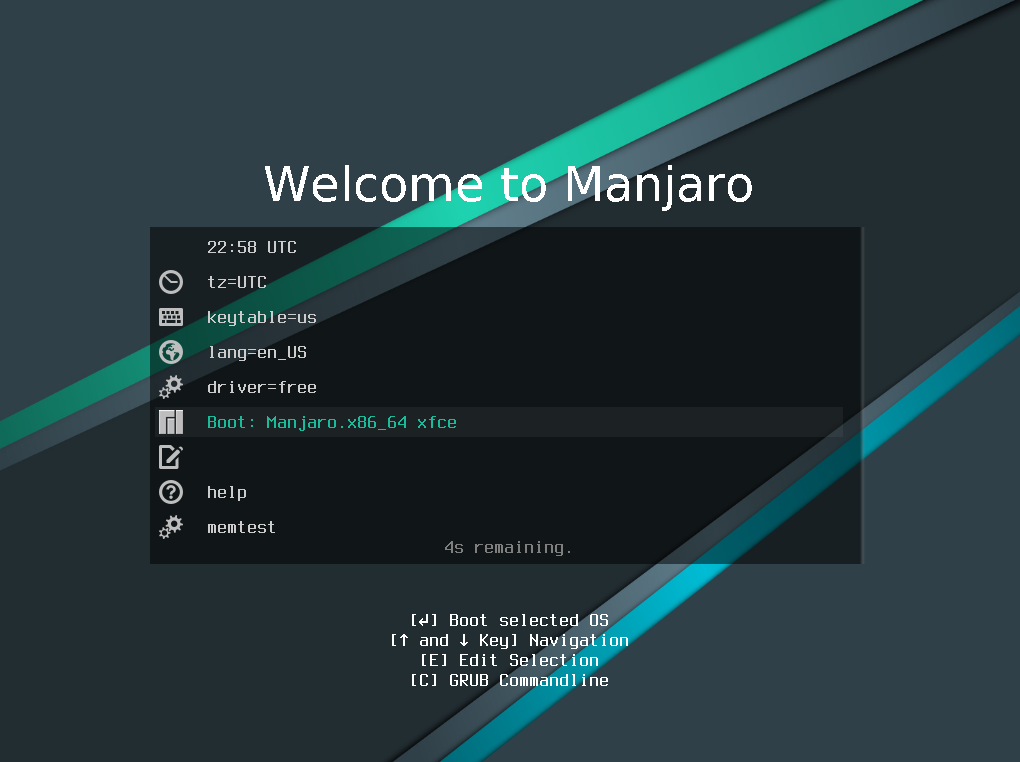
\includegraphics[width=0.6\textwidth, center]{manjaro_install1.png}

\item \textbf{Live USB} \par
W tym momencie jesteśmy w środku środowiska instalacyjnego. Możemy tu sprawdzić jak wizualnie będzie wyglądał system, jakie będziemy mieli opcje konfiguracji czy też jak nam się używa taki interfejs. Gdy już skończysz oględziny i uznamy, że chcemy kontynuować wybieramy instalator z pulpitu i przechodzimy dalej.\\

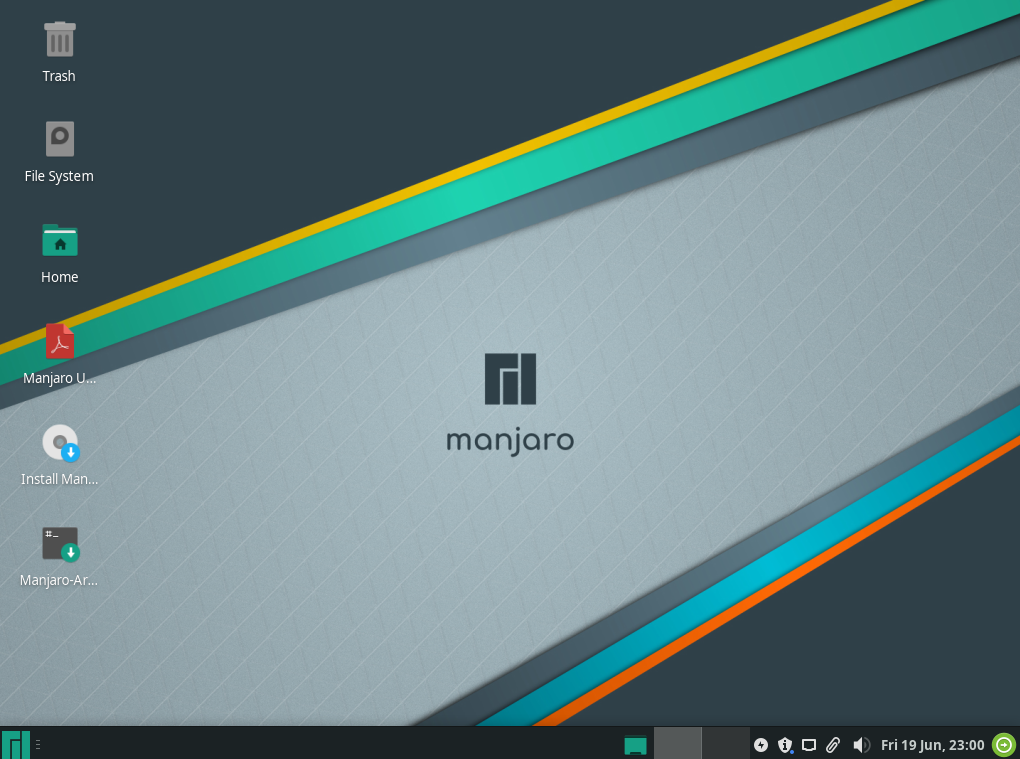
\includegraphics[width=0.75\textwidth, center]{manjaro_install2.png}



\item \textbf{Instalator} \par
Wiele dystrybucji posiada polskie instalatory co ułatwi proces osobą z mniejszym zrozumieniem języka angielskiego. Każdy też ma swoje specyficzne etapy, które charakteryzują różne dystrybucje.\\

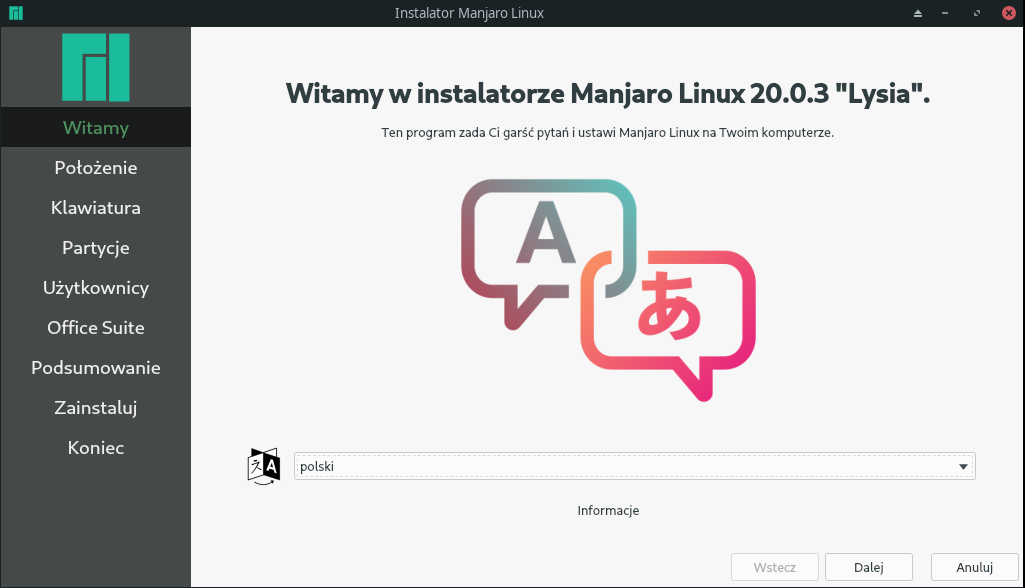
\includegraphics[width=0.95\textwidth, center]{manjaro_install3.png}\\\\\\

\item \textbf{Wybór strefy czasowej} \par
Aby upewnić się, że czas systemowy jest taki sam jak czas na twoim zegarku musimy ustawić strefę czasową dla servera NTP.\\

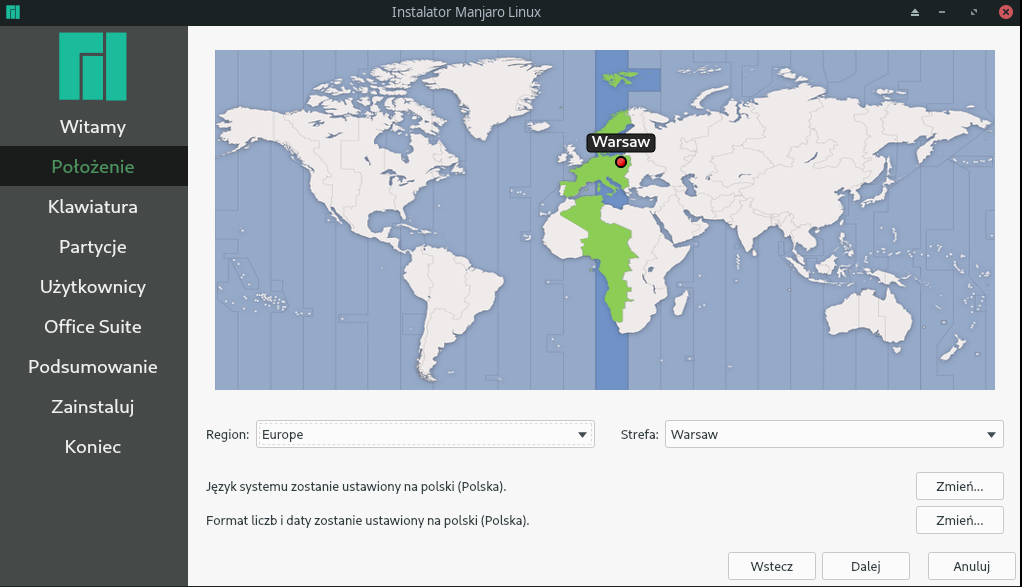
\includegraphics[width=0.95\textwidth, center]{manjaro_install4.png}\\\\\\



\item \textbf{Klawiatura} \par
Jeśli masz w imieniu lub po prostu zamierzasz użyć polskich znaków lub innych niedostępnych na standardowej klawiaturze angielskiej, wybierz układ odpowiedni do twoich potrzeb.\\

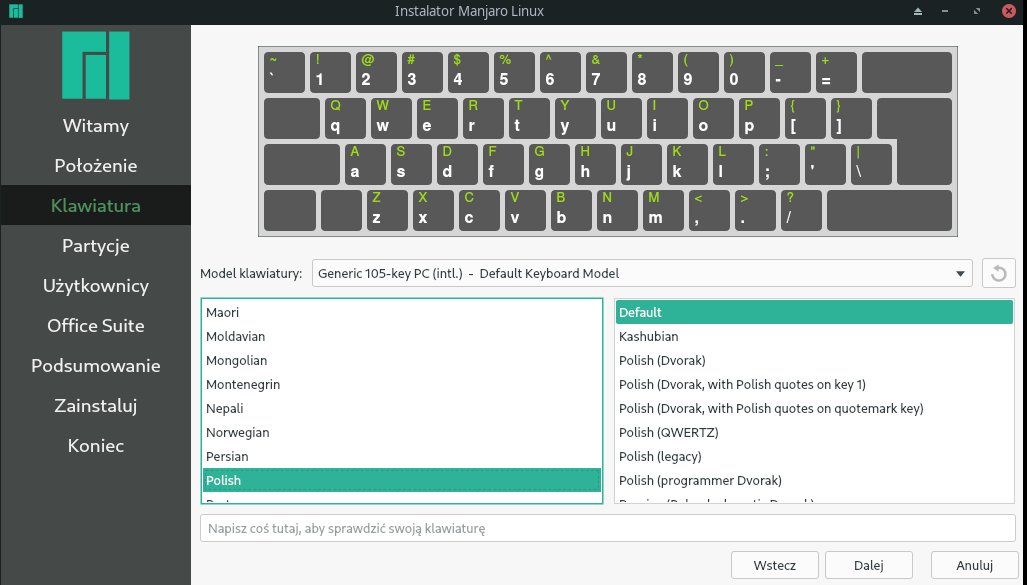
\includegraphics[width=0.95\textwidth, center]{manjaro_install5.png}\\\\\\

\item \textbf{Partycjonowanie} \par
Jest to najważniejszy etap instalacji. Tutaj czyścisz dysk aby zrobić miejsce na nowy system lub tworzysz odpowiednie środowisko z dostępnego miejsca. Dużo instalatorów posiada opcje domyślne, niewymagające własnego wkładu w partycjonowanie. Jeśli jednak nie masz takiej opcji poczytaj dokładnie poradniki do instalacji twojej dystrynbucji.\\

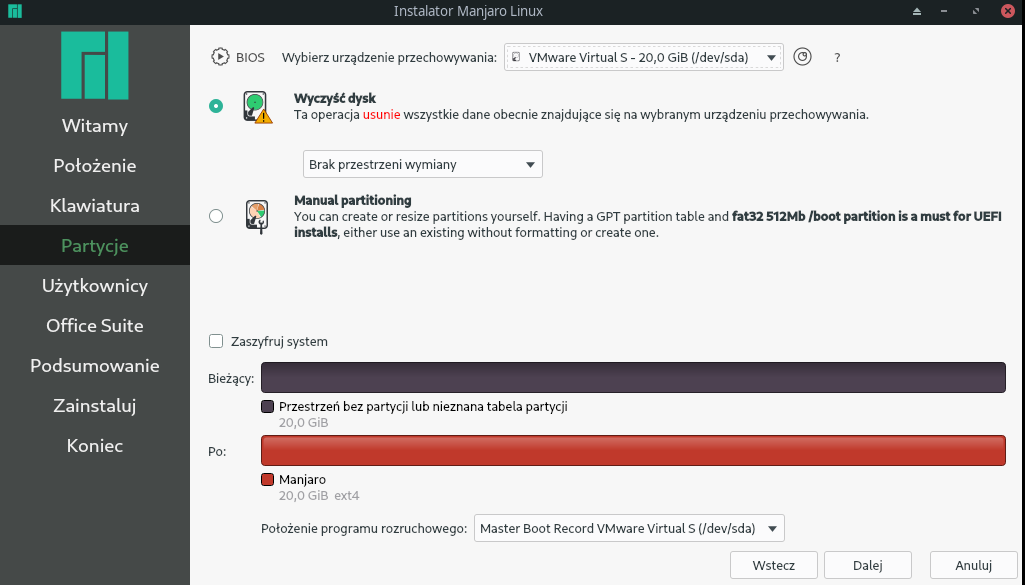
\includegraphics[width=0.95\textwidth, center]{manjaro_install6.png}\\\\\\



\item \textbf{Tworzenie kont administratora i użytkownika} \par
Aby skorzytać z systemu potrzebujemy konta umożliwiającego dostęp do niego. Podczas instalacji zawsze tworzymy konto administratora "root", które posiada wszelkie uprawnienia na maszynie. Stosunkowa większość dystrybucji wymaga utworzenia także konta upoważnionego, mającego dostęp do wykonywania operacji administratora ale posiadające inne hasło niż sam administrator. Pomaga to zwiększyć bezpieczeństwo.\\

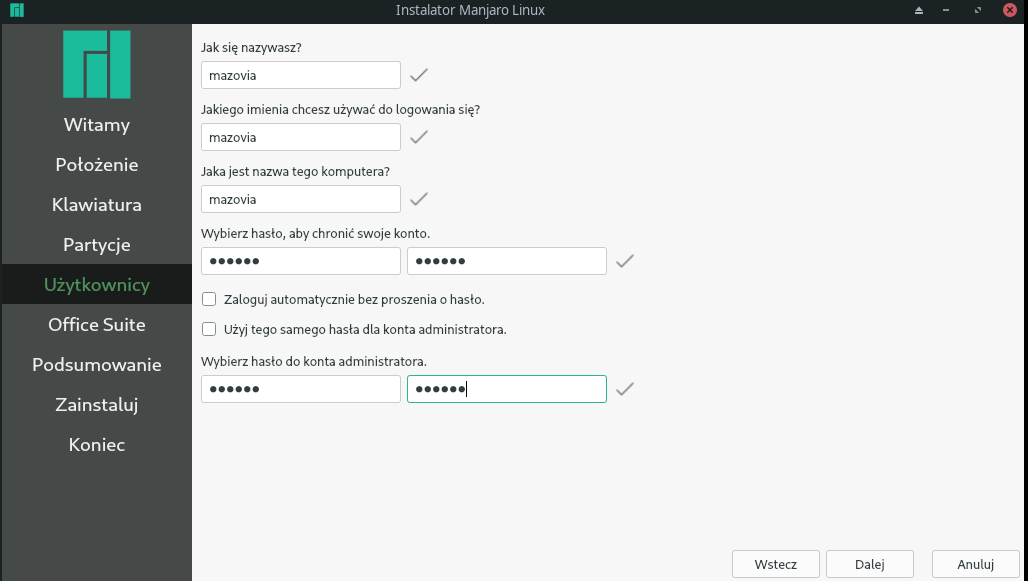
\includegraphics[width=0.95\textwidth, center]{manjaro_install7.png}\\\\\\

\item \textbf{Dodatkowe opcje} \par
Różne dystrybucje posiadają różne dodatkowe opcje poprawiające wrażenia zaraz po instalacji. Głównie dotyczą wyboru pakietów aplikacji oraz konfiguracji serwisów.\\

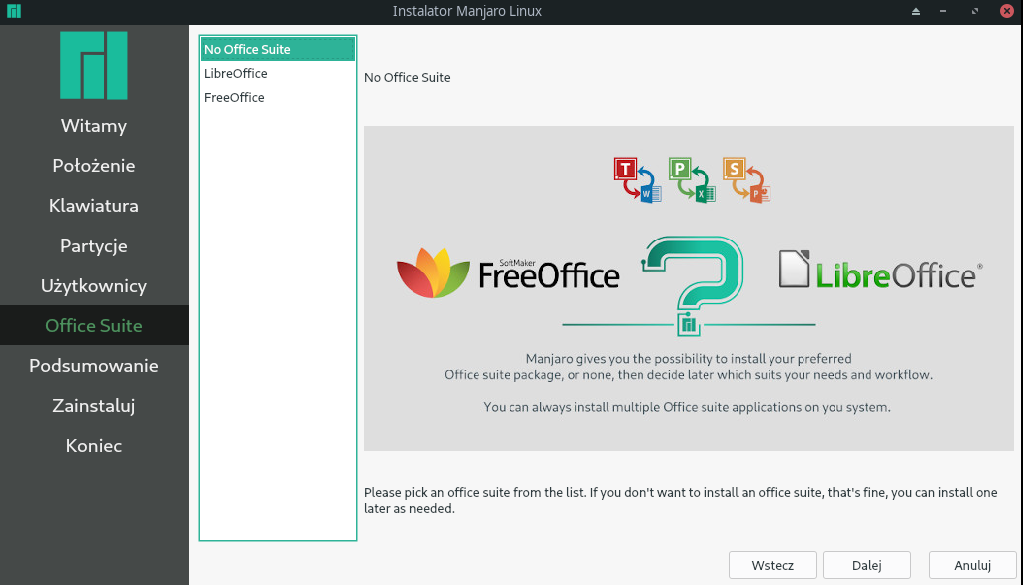
\includegraphics[width=0.95\textwidth, center]{manjaro_install8.png}\\\\\\




\item \textbf{Podsumowanie} \par
Tutaj upewnij się, że wszystkie elementy instalcji są takie same jak wybrany wcześniej. Po uruchomiueniu instalatora nie będzie można dokonać żadnych zmian. Wiąże się to też z utratą danych na dysku wiec upewnij się, że masz kopię zapasową plików ważnych dla ciebie. Jeśli jednak po instalcji okaże się, że wybrana opcja była inna niż zamierzana, a dotyczy ona samego systemu operacyjnego to po prostu uruchom instalator ponownie, tym razem wybierając odpowiednio.\\

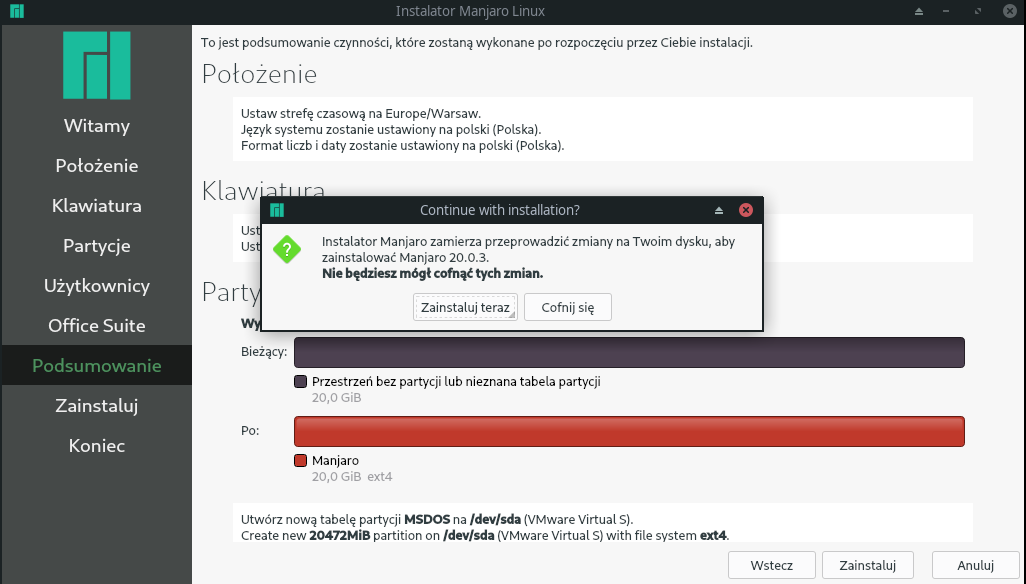
\includegraphics[width=0.9\textwidth, center]{manjaro_install11.png}\\\\

\item \textbf{Zakończenie} \par
Gdy już udało ci się poprawnie zainstalować Linuxa musisz uruchomić komputer ponownie, żeby móc korzytać z nowego systemu. Pamiętaj, że przed uruchomieniem się komputera warto wyjąć pendriva. Ułatwia to maszynie rozpoznanie dysku zawierającego system.\\

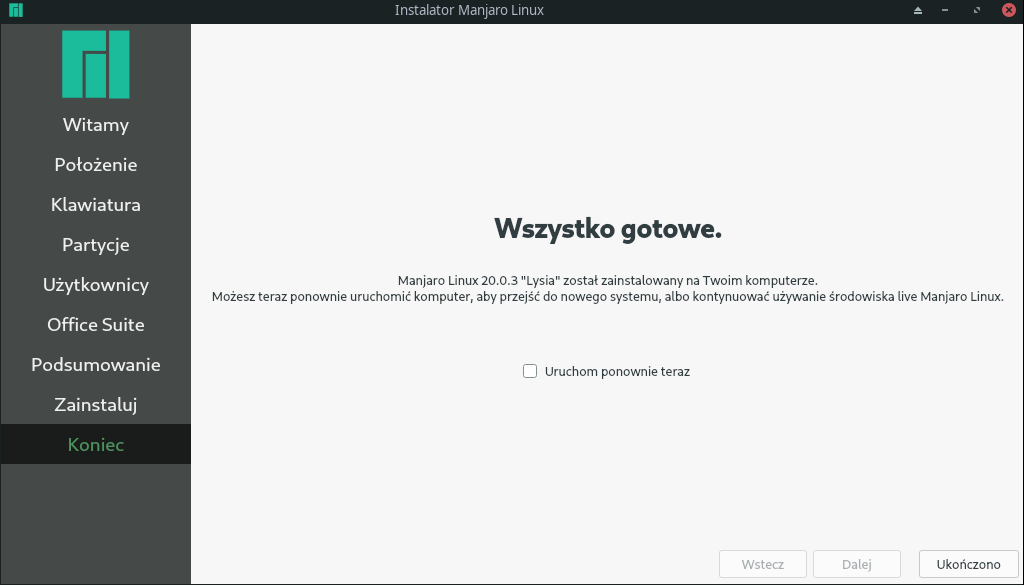
\includegraphics[width=0.9\textwidth, center]{manjaro_install13.png}\\\\\\

\end{enumerate}
 
\subsection{Konfiguracja poinstalacyjna}	

Nie każda dystrybucja jest gotowa do użytku zaraz po zainstalowaniu, a nawet te które są wciąż posiadają swoje mankamenty i małe rzeczy poprawiające wrażenia. Aby znaleźć listę takich rzeczy po prostu wyszukaj "[twoja dystrybucja] post install". Jednak jeśli nie chcesz marnować czasu na szykanie informacji przedstawiam tutaj parę najważniejszych ustawień wartych uwagi.

\begin{enumerate}

\item \textbf{Zaktualizuj system} \par Aby mieć pewność, że system jest w swojej najnowszej wersji warto zaraz po instalacji wykonać sprawdzenie aktualizacji przy pomocy wbudowanego programu. Możesz także wpisać komendy wykonujące wszystko za ciebie
\begin{itemize}
\item \textbf{Rodzina Debiana i Ubuntu} (menager pakietów APT) - \textsl{\underline{sudo apt update \&\& sudo apt upgrade -y}}
\item \textbf{Arch oraz Manjaro} (menager pakietów Pacman) - \textsl{\underline{sudo pacman -Syyu}}\\
\end{itemize}

\item \textbf{Zainstaluj sterowniki}\par Upewnij się, że wszystkie sterowniki są zainstalowane w swojej najnowszej wersji. Ich brak może wiązać się z dużymi problemami z konkretnym urządzeniem. Zapewnia to też najlepszą wydajność i stabilność.\\

\item \textbf{Zainstaluj kodeki multimedialne} Aby móc odtwarzać najróżniejsze formaty wideo i audio warto zainstalować kodeki odpowiadające za ich przetwarzanie. Można tego dokonać tą komendą choć na twoim systemie może się różnić:
\begin{itemize}
\item \textsl{\underline{sudo apt-get install ubuntu-restricted-extras}}\\
\end{itemize}

\item \textbf{Zarządzanie baterią} \par Najważniejsza opcja dla użytkowników laptopów to zestaw narędzi do zarządzania energią. Pakiet najbardziej rozbudowany i naczęściej używany to \textbf{TLP}. Pozwala znacząco poprawić żywotność laptopa oraz monitorować pobór mocy. Można go zainstalować komendą:
\begin{itemize}
\item \textsl{\underline{sudo apt install tlp tlp-rdw \&\& sudo tlp start}}\par
\end{itemize}
Aby zapoznać się z wszystkimi aspektami tego usprawnienia warto przeczytać dokumentację twórców:\\\url{https://linrunner.de/tlp/introduction.html}\\

\item \textbf{Zmniejszenie preferencji użycia pliku wymiany}\par Jeśli twoja maszyna ma powyżej 4 GB ramu to może się okazać, że system nie jest tak szybki jak mógłby być. Związane jest to z względnie agresywnym ustawienium użycia pliku wymiany zamiast pamięci RAM. Aby zapewnić szybsze działanie wystarczy zmienić wartość tej preferecji w plikach konfiguracyjnych takimi komendami:
\begin{itemize}
\item \textsl{\underline{sudo sysctl vm.swappiness=10}}\\\\\\\\
\end{itemize}

\end{enumerate}

	\section{Nauka obsługi systemu oraz dobre nawyki}
	

	
\chapter{Aplikacje i środowiska alternatywne}

VLC – media player for videos
GIMP – Photoshop alternative for Linux
Pinta – Paint alternative in Linux
Calibre – eBook management tool
Chromium – Open Source web browser
Kazam – Screen recorder tool
Gdebi – Lightweight package installer for .deb packages
Spotify – For streaming music
Skype – For video messaging
Kdenlive – Video editor for Linux
Atom – Code editor for programming
Android Studio –  For Android app development

	\section{Biurowe}
	
	\section{Software Development}
	
	\section{Twórczość}
	
	\section{Inne}
	
\chapter{Automatyzacja zadań}

	\section{Metody automatyzacji}
	
	\section{Przykładowe programy i źródła}
	
\chapter{Linux i Gaming?}

	\section{Problemy z linuxem}
	
	\section{Rozwiązania społeczności}
	
\chapter{Bezpieczeństwo}

	
\chapter{Podsumowanie}

	\section{Zalety i wady}
	
	\section{Dodatkowe materiały merytoryczne do wglądu własnego}
	
\chapter{Zakończenie}
\newpage \newpage
\chapter{Źródła}
\end{document}
